\subsection{Pipelining}
\label{sub:pipelining}


\begin{figure}
\begin{minted}{c}
#pragma omp target teams distribute\
  pipeline(static)\
  map(pipeline,to:A[k-1:3][0:ny][0:nx])\
  map(pipeline,from:An[k:1][0:ny][0:nx])
for(k=1;k<nz;k++) {
  #pragma omp parallel for
  for(i=1;i<nx;i++) {
    for(j=1;j<ny;j++) {
      An[Index3D (i,     j,     k)] =
      (A[Index3D (i,     j,     k + 1)] +
       A[Index3D (i,     j,     k - 1)] +
       A[Index3D (i,     j + 1, k)] +
       A[Index3D (i,     j - 1, k)] +
       A[Index3D (i + 1, j,     k)] +
       A[Index3D (i - 1, j,     k)])*c1
     - A[Index3D (i,     j,     k)]*c0;
    }
  } 
}
\end{minted}
\caption{Example of a possible syntax for pipelining a stencil loop.\label{fig:Cancellation}}
\end{figure}

\begin{figure}
  \centering
  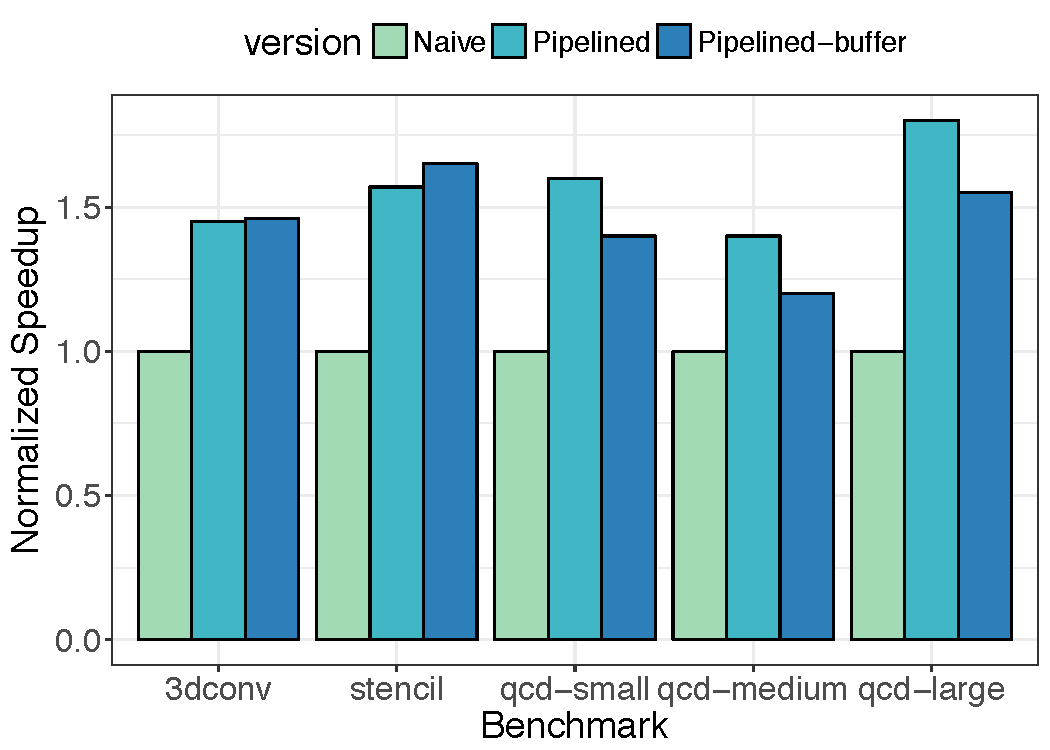
\includegraphics[width=0.5\textwidth]{pics/pipelining-perf}
  \caption{Speedup of pipelined or pipelined with buffering, memory limited
  pipelining, data transfer across kernels.\label{pipeline-perf}}
\end{figure}

